%%%%%%%%%%%%%%%%%%% READ ME%%%%%%%%%%%%%%%%%%%%%%%%
% This file is only used for compilation of the final report by the editors and thus should NOT BE CHANGED, EXCEPT for putting in your title and author names below. All text, figures, tables etc are supposed to be written in the according section files in the "sections" subfolder. IF YOU END UP NOT NEEDING a separate summary and/or appendix section, COMMENT OUT BELOW in the \input{} lines accordingly (also see the comments below and do the same thing in "COMPILE_REPORT.tex")! The "preamble_single" holds a comprehensive selection of packages and custom settings commonly used and useful for scientific reports. Only add packages if really needed and best do so at the end of the "preable_single" file - and let the final report editors know, if you added anything to make their life easier. Also, if in doubt about general formatting choices, talk to the other groups and the editor team to ensure uniform style throughout the final report.
%%%%%%%%%%%%%%%%%%%%%%%%%%%%%%%%%%%%%%%%%%%%%%%%%%%%%%%%%%%%%%
\begin{document}

% Put in your report title here (also put it in "COMPILE_REPORT.tex")
\chapter{Report title}

% Put in your author names here (also put them in in "COMPILE_REPORT.tex")
\chapterauthor{Author 1, Author 2}

% Here the indivual sections are incorporated for compilation. If you end up not having a separate summary/conclusion and/or report, comment out one or both lines below accordingly (also, do the same thing in "compile.tex")!
\begin{abstract}

Put your abstract here.

\end{abstract}
\section{Introduction} \label{sec:introduction}

Put your introduction here. Cite literate as \cite{ArcticAmplification} or \citep{ArcticAmplification}.
\section{Instruments, Data and Methods} \label{sec:methods}

\subsection{Darcy's law}

Darcy's law describes the hydraulic flux of a fluid through a cross section using the hydraulic conductivity.\\
Without gravitational influence the instantaneous flux $q[m/s]$ though a porous medium with cross section $A[m^2]$ and permeability $k[m^2]$ of a fluid with viscosity $\mu[Pa \; s]$ is given by equation \ref{darcys law}

\begin{equation}\label{darcys law}
    q = -\frac{k}{\mu}\nabla p
\end{equation}

Where $\nabla p[Pa]$ is the pressure gradiant over the volume.
The negative sign means that the fluid flows from high pressure area to a low pressure area.
In the case of vertical flux and by assuming a hydrostatic pressure we can relate the pressure to the height of the fluid by Stevin's law.
We then consider the seawater to be incompressible and the height of the hole to be negligible compared to the radius of the earth, so that $g$ and $\rho$ can be assumed constant.

\begin{equation}\label{darcyslawdiffeq}
    q(t) = -\frac{\rho g k}{\mu L}\Delta h(t) \\
\end{equation}

Where $g$ is the gravitational acceleration, $\rho$ is the density of the fluid and $L[m]$ is the distance the fluid percolates.
Note that we have added a time dependency of the height and thus flux.
Darcy's law does not account for a change in pressure, but as our holes fills with water the height and pressure changes, altering the flux.
Only when the pressure gradient is fairly large we are able to compute the permeability, when the gradient goes towards zero the equation is no longer valid.  \\
We assume the other parameters to remain constants.
The solution to the first-order linear ordinary differential equation \ref{darcyslawdiffeq} is given on the form:

\begin{equation}
    y(t) = A \: \frac{d}{dt}\left( y(t) \right) \Rightarrow y(t) = c_1 \: e^{\frac{t}{A}}
\end{equation}

The solution shows an exponential relation between height and time.

\begin{equation}\label{diff eq solution}
    h(t) = h_0 \: exp\left(-\frac{\rho g k t}{\mu L}\right)
\end{equation}

Linearizing and solving for the permeability $k$ yields:

\begin{equation}\label{lin.diff sol}
    k = -a\frac{\mu L}{\rho g}
\end{equation}

Were as $a$ is a linear relation coefficient defined as $a = \log\left(\frac{h(t)}{h_0}\right) /t$ which can be found by regression.

\subsection{Empirical model}





\section{Results} \label{sec:results}

Put your results here.

% This is a dummy figure following "best practice"
\begin{figure}[thbp]
    \centering
    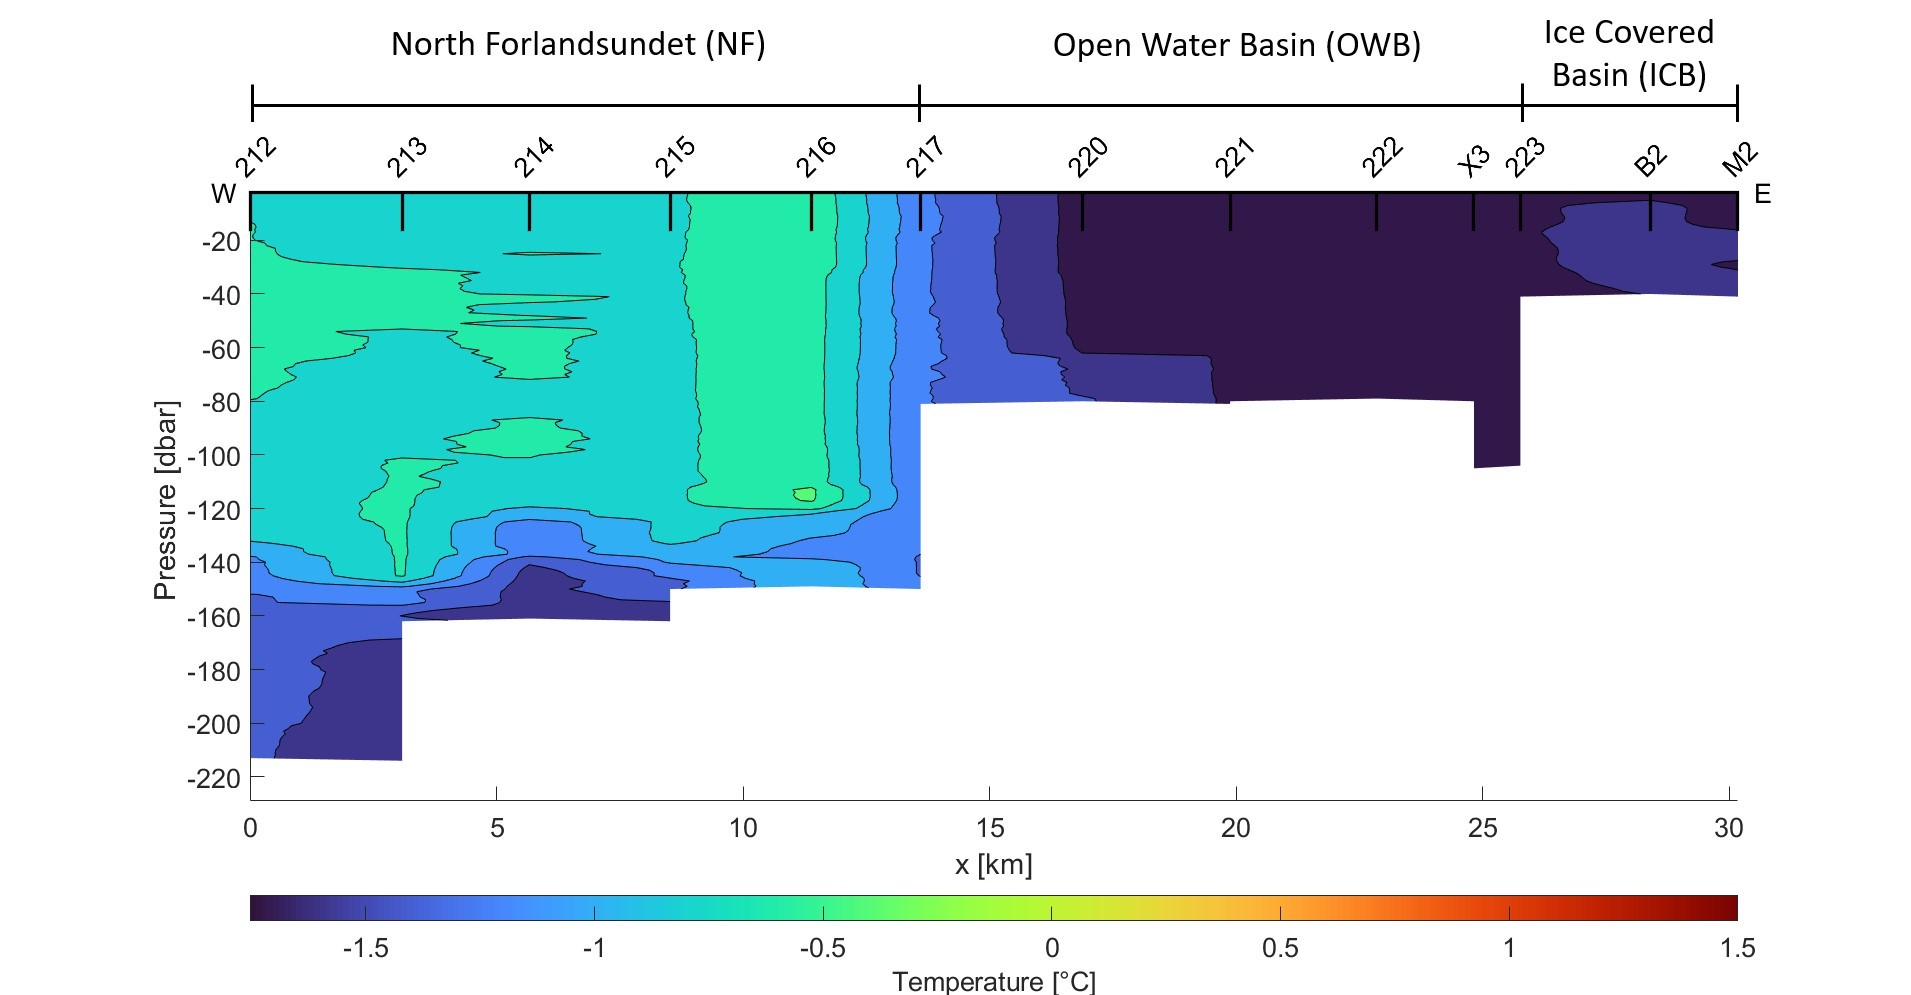
\includegraphics[width=\textwidth]{report_template/figures/dummy-figure.jpg}
    \caption{Caption of the dummy figure}
    \label{fig:dummy_figure}
\end{figure}


VI SÅ JO VELDIG MYE MERE WATER PONDS DAGENE ETTER, FORDI FERSK LAGET HAR SMELLTET OG PERMABILITET ØKTE, SÅ DEN KOM MERE VANN OPP
\section{Discussion} \label{sec:discussion}

Put your discussion here. Your conclusion could be included in this part, or given in the extra "05\_discussion.tex" file. Remember to include or exlude the files (comment or uncomment) in "COMPILE\_REPORT.tex" and "main.tex" accordingly!
\section{Summary} \label{sec:summary}

Put your summary/conclusion here, if it is not included in the discussion section. Remember to include or exlude the files (comment or uncomment) in "COMPILE\_REPORT.tex" and "main.tex" accordingly!

% This inputs the bibliography of your report
\bibliography{literature}
\bibliographystyle{AGFstyle}

% Appendix usually goes behind the bibliography (comment out, if you do not have any)
\section{Appendix} \label{sec:appendix}

Put your appenx here, if you have any. Remember to include or exlude the files (comment or uncomment) in "COMPILE\_REPORT.tex" and "main.tex" accordingly!

If you have multiple appendices and want to structure them, you can use subsections as bellow!

\subsection{Appendix 1}
Put appendix 1 here.

\subsection{Appendix 2}
Put appendix 1 here.